\title{A grammar of {Gyeli}}
\author{Nadine Grimm}
\renewcommand{\lsSeries}{cogl}%use series acronym in lower case

\dedication{\normalfont\Large
\textit{Púù yá bámbámbɔ́ bísì bà vú mɔ̀ bî ---}\\
\textit{yá bálɛ́ɛ̀ mápè'è máwɔ̀}\\

\textit{For our ancestors who have left us ---}\\
\textit{may we keep their wisdom}\\

\vfill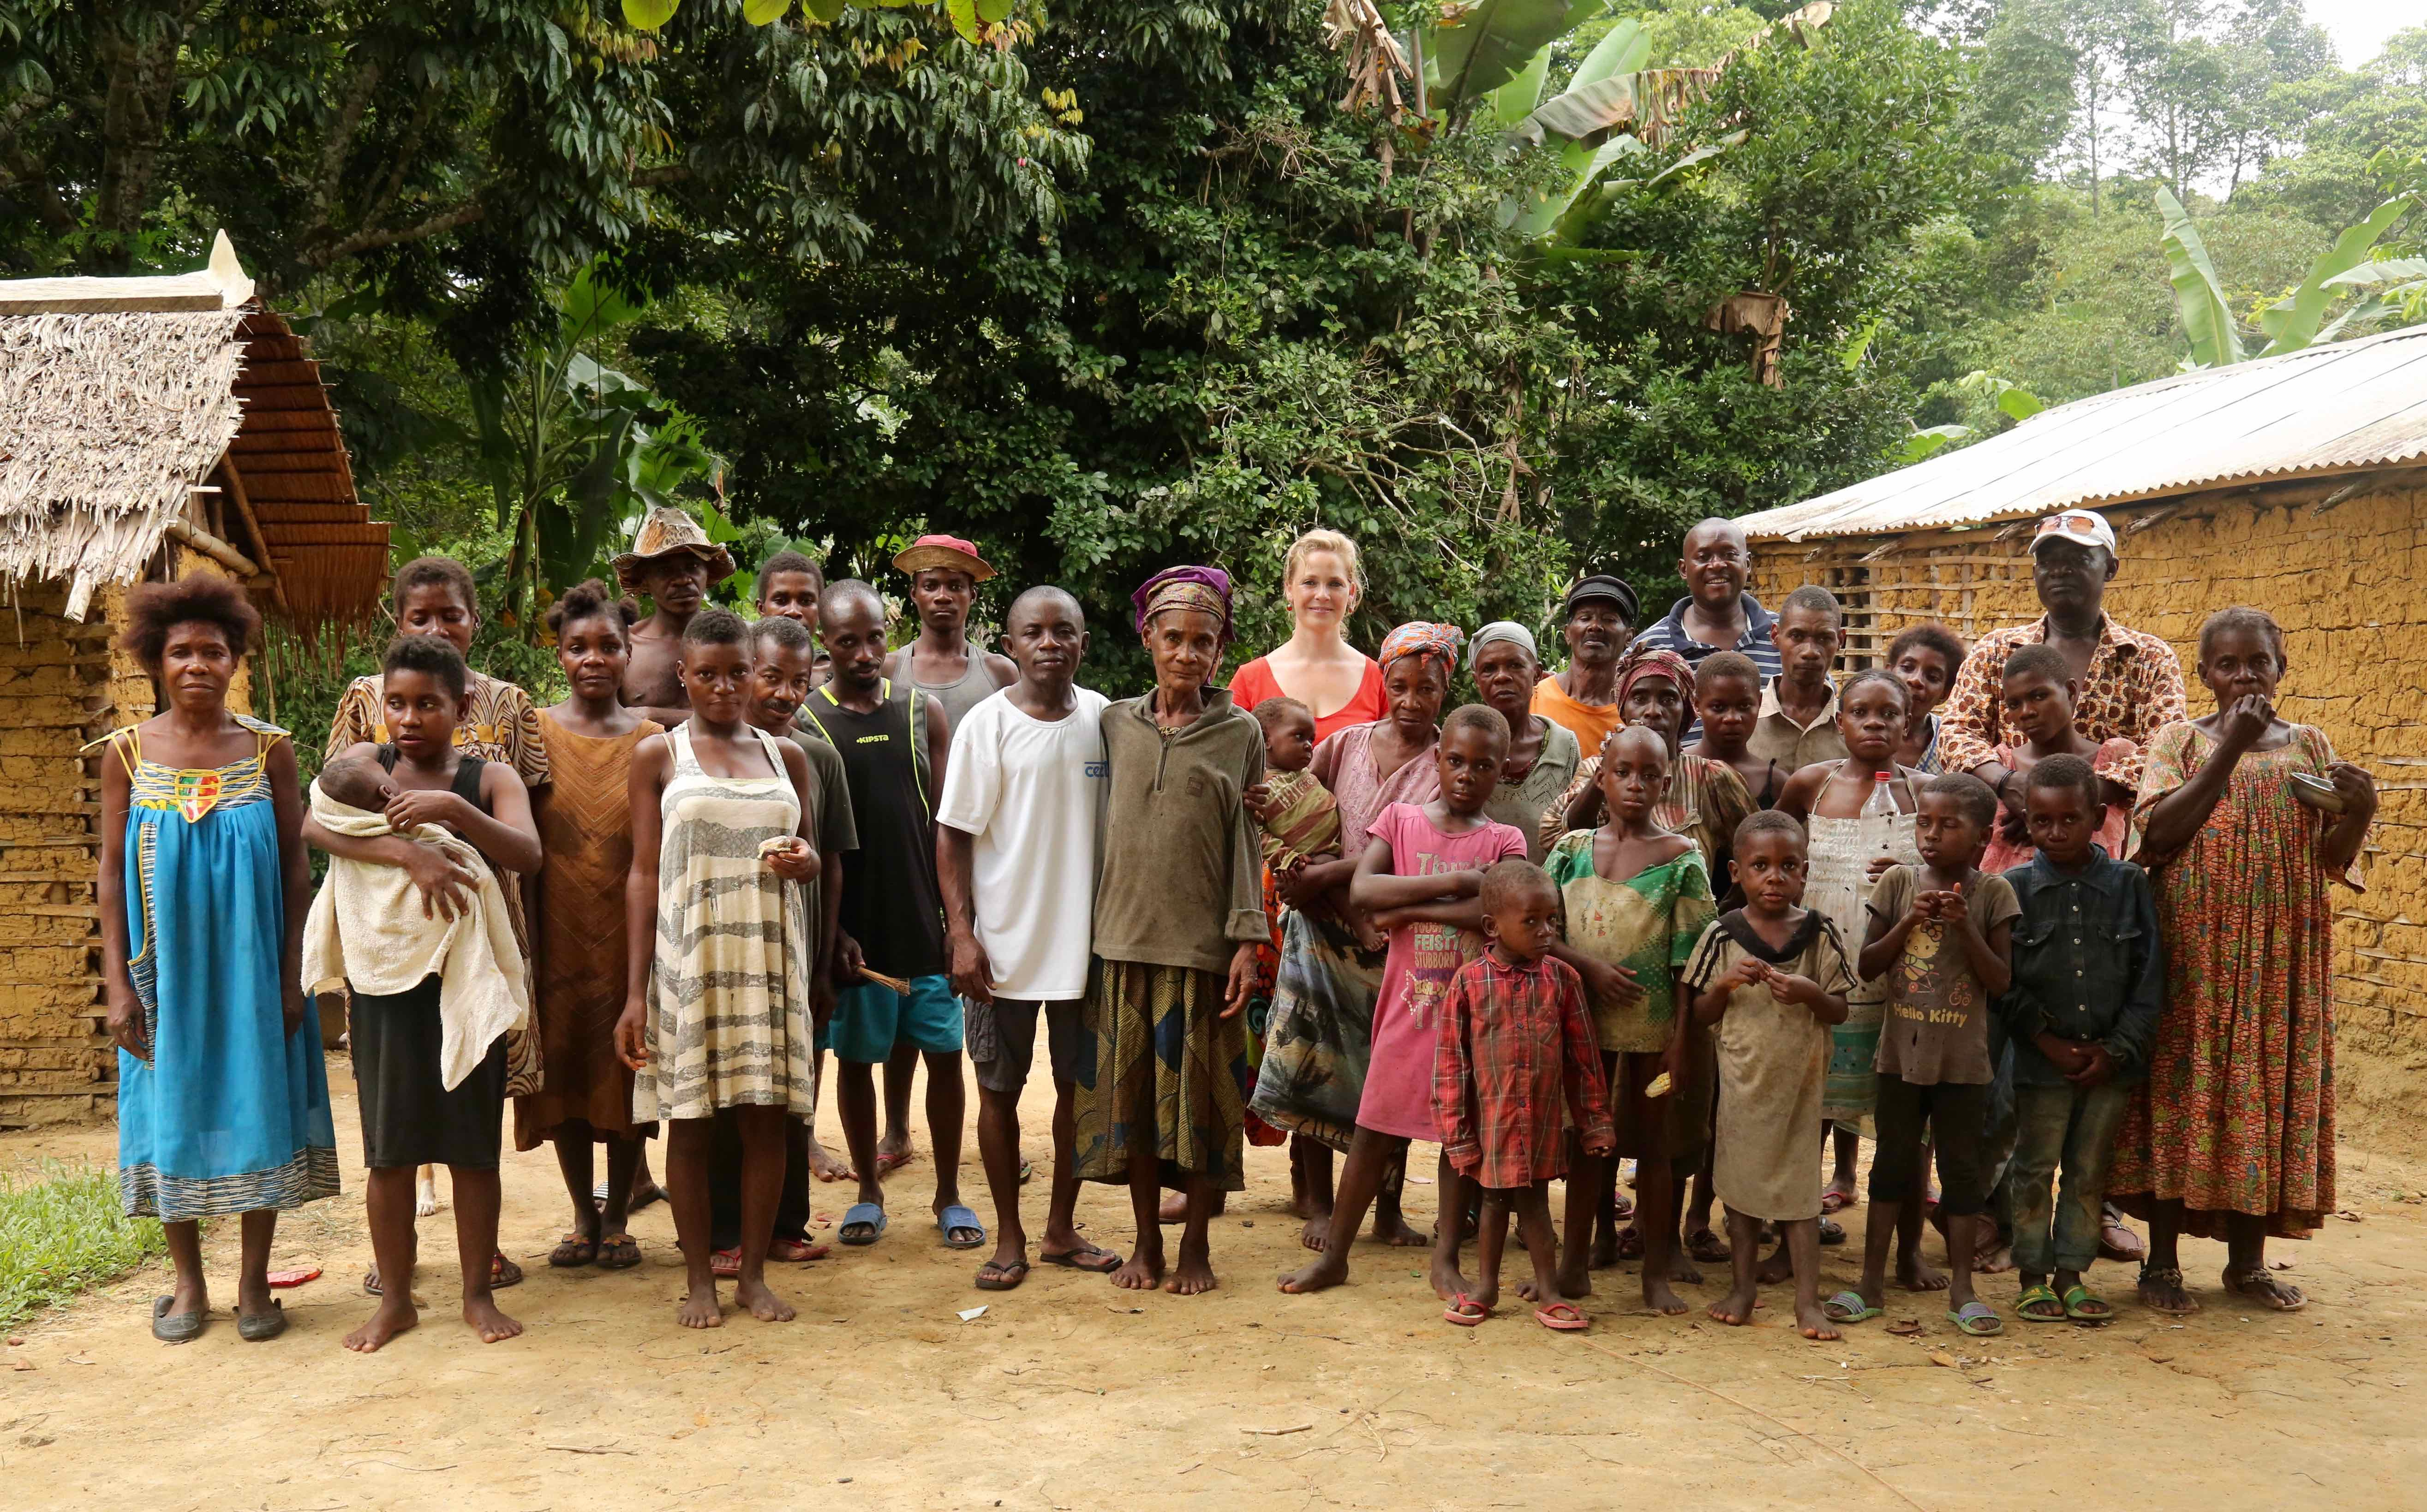
\includegraphics[width=\textwidth]{figures/Bagyeli-Ngolo.jpg}\vfill}

\BookDOI{10.5281/zenodo.4737370}
\renewcommand{\lsISBNdigital}{978-3-96110-311-9}
\renewcommand{\lsISBNhardcover}{978-3-98554-007-5}

\renewcommand{\lsSeriesNumber}{2}
\renewcommand{\lsID}{298}

\renewcommand{\lsImpressumExtra}{This book is the revised version of the author's PhD dissertation which was accepted by the Faculty of Humanities and Social Sciences at Humboldt University of Berlin in 2015.}

\BackBody{This grammar offers a grammatical description of the Ngòló variety of Gyeli, an endangered Bantu (A80) language spoken by 4,000--5,000 ``Pygmy'' hunter-gatherers in southern Cameroon. It represents one of the most comprehensive descriptions of a northwestern Bantu language.

The grammatical description, which is couched in a form-to-function approach, covers all levels of language, ranging from Gyeli phonology to its information structure and complex clauses.

It draws on nineteen months of fieldwork carried out as part of the ``Bagyeli/Bakola'' DoBeS (documentation of endangered languages) project between 2010 and 2014. The resulting multimodal corpus from that project, which includes texts of diverse genres such as traditional stories, narratives, multi-party conversations and dialogues, procedural texts, and songs, provides the empirical basis for the grammatical description. The documentary text collection, supplemented by data from elicitation work, questionnaires, and experiments, are accessible in the Bagyeli/Bakola collection of the Language Archive. With additional ethnographic, sociolinguistic, diachronic, and comparative remarks, the grammar may appeal to a wider audience in general linguistics, typology, Bantu studies, and anthropology.

In 2019, the grammar received the Pāṇini Award by the Association for Linguistic Typology.}

\typesetter{Nadine Grimm, Felix Kopecky, Sebastian Nordhoff}

\proofreader{Alexandra Fosså,
Amir Ghorbanpour,
Brett Reynolds,
Christian Döhler,
Craevschi Alexandru,
Franny Vandervoort,
Gereon A. Kaiping,
James Gray,
Jeroen van de Weijer,
Konstantinos Sampanis,
Lachlan Mackenzie,
Ludger Paschen,
Marten Stelling,
Matthew Windsor,
M. Chiara Miduri,
Madeline Myers
Mykel Brinkerhoff,
Russell Barlow,
Tihomir Rangelov,
Yvonne Treis
}
